\chapter{Metode Penelitian}
Secara umum, tujuan dari penelitian ini adalah mengembangkan model SQR dengan \emph{watermark} yang dapat diautentikasi. Penelitian ini juga menguji
efektivitas CDP 2 dan 4 level berdasarkan akurasi autentikasinya. Selain itu, penelitian ini juga menguji efektivitas penggunaan penanda ArUco dalam
melokalisasi objek CDP. Terakhir, penelitian ini juga mencarai parameter P\&S yang tepat dalam pembuatan \emph{dataset} SQR seperti konfigurasi kamera serta
jenis kertas dan tinta yang digunakan untuk mencetak SQR, sehingga mendapatkan hasil akurasi autentikasi yang tinggi. Dalam prosesnya, metode-metode penelitian
yang dirancang dan dilakukan penulis akan dijelaskan pada bab ini.

\section{Alat dan Bahan Tugas Akhir}

\subsection{Alat Tugas Akhir}

Alat yang digunakan pada penelitian ini terbagi atas perangkat keras dan perangkat lunak yang dengan rincian sebagai berikut:

\begin{enumerate}
	\item Laptop Lenovo Legion Y530\\Merupakan perangkat keras utama yang digunakan dalam penelitian. Laptop ini memiliki spesifikasi sebagai berikut: Prosesor Intel
	      I5-8300H, RAM 8 GB DDR4, dan kartu grafis Nvidia Geforce GTX 1050TI (4 GB).
	\item Python 3.9\\Perangkat lunak yang merupakan bahasa pemrograman utama yang digunakan dalam mengembangkan model SQR, pengolahan data, dan membuat model untuk
	      mengautentikasi SQR.
	\item AutoGluon\\Merupakan pustaka AutoML sumber terbuka yang mengotomasi pembuatan model \emph{deep learning} (DL) dan \emph{machine learning} (ML) untuk
	      menyelesaikan permasalahan di dunia nyata yang melibatkan \emph{dataset} gambar, teks, dan tabular. AutoGluon dapat menyederhanakan alur kerja pembuatan model
	      yang biasanya kita lakukan. Dengan AutoGluon, kita dapat mengembangkan dan memperbaiki model hanya dengan mengoptimasi parameter dengan beberapa baris kode
	      saja.
	\item Microsoft Visual Studio Code\\Merupakan salah satu perangkat lunak editor kode sumber terpopuler dan gratis yang dikembangkan oleh Microsoft. Editor ini
	      memiliki berbagai fitur yang memungkinkan pengguna untuk menulis, mengedit, dan mengelola kode sumber dengan mudah dan efisien. Selain itu, editor ini juga
	      mendukung berbagai bahasa pemrograman, termasuk JavaScript, Python, Java, C++, dan masih banyak lagi. Tampilan antarmuka pengguna VS Code sangat bersih dan
	      dapat disesuaikan, sehingga pengguna dapat mengatur tata letak dan tema yang sesuai dengan preferensi mereka. Selain itu, editor ini juga mendukung berbagai
	      bahasa pemrograman, termasuk JavaScript, Python, Java, C++, dan masih banyak lagi. Fitur-fitur kunci dari VS Code termasuk kemampuan untuk mengeksekusi kode
	      secara langsung dari editor, penyelesaian otomatis kode, refaktoring kode, debugging, pengelolaan paket, dan integrasi dengan sistem kontrol versi seperti Git.
	\item Ekstensi Jupyter Notebook untuk VS Code\\Merupakan ekstensi yang dimiliki oleh Microsoft Visual Studio Code untuk menjalankan \emph{notebook} di dalam
	      \emph{environment} Microsoft Visual Studio Code.
	\item Adobe Acrobat DC\\Merupakan perangkat lunak yang digunakan sebagai pembaca dan pengedit fail PDF. Perangkat lunak ini banyak penulis gunakan untuk mengubah
	      ukuran \emph{batch} QR menjadi ukuran standar percetakan.
	\item Adobe Photoshop 2022\\Merupakan perangkat lunak yang digunakan sebagai editor gambar. Perangkat lunak ini penulis gunakan dalam penelitian untuk mengubah fail
	      PNG hasil \emph{generate batch} QR dari kode menjadi PDF.
	\item \emph{Smartphone} Realme GT Neo 3T\\Perangkat keras yang digunakan sebagai pemindai SQR dalam pembuatan \emph{dataset} SQR orisinal dan palsu. \emph{Smartphone} ini memiliki spesifikasi sebagai berikut: \emph{Chipset} Qualcomm SM8250-AC Snapdragon 870 5G, sistem operasi Android 12, kamera utama dengan resolusi 64 MP, f/1.8, 25mm.
	\item \emph{Printer} Xerox Versant\\Perangkat keras yang digunakan sebagai pencetak utama \emph{dataset} SQR orisinal dan palsu. \emph{Printer} ini merupakan \emph{printer} berspesifikasi tinggi yang banyak digunakan dalam industri percetakan.
	\item Boks\\Boks digunakan sebagai \emph{environment} yang digunakan untuk menstandarisasi hasil pemotretan atau pemindaian \emph{dataset} SQR menggunakan kamera
	      \emph{smartphone}.
	\item Gunting\\Gunting digunakan untuk memotong \emph{dataset} SQR yang nantinya akan dipotret.
\end{enumerate}

\subsection{Bahan Tugas akhir}

Bahan yang digunakan pada penelitian secara garis besar merupakan \emph{dataset} SQR dengan rincian sebagai berikut:

\begin{enumerate}
	\item \emph{Dataset} SQR 2 Level \emph{Grayscale}\\\emph{Dataset} SQR 2 dengan 2 level \emph{grayscale} terdiri dari 200 \emph{dataset} foto pertama (orisinal) dan 200 \emph{dataset} foto kedua (palsu).
	\item \emph{Dataset} SQR d4 Level \emph{Grayscale}\\\emph{Dataset} SQR dengan 4 level \emph{grayscale} terdiri dari 200 \emph{dataset} foto pertama (orisinal) dan 200 \emph{dataset} foto kedua (palsu).
	\item \emph{Dataset} SQR untuk Pengujian Parameter\\\emph{Dataset} ini digunakan untuk melakukan verifikasi parameter pembuatan model SQR, pemotretan, dan pencetakan SQR, misalnya ukuran penanda ArUco, ukuran SQR, ukuran CDP, konfigurasi kamera, serta jenis kertas dan tinta yang digunakan untuk mencetak SQR.
\end{enumerate}

\section{Metode yang Digunakan}
Penelitian ini termasuk ke dalam penelitian kuantitatatif yang dilakukan dengan eksperimen. Eksperimen yang dilakukan adalah dengan melakukan verifikasi
parameter yang akan digunakan dalam pembuatan SQR, pembuatan \emph{dataset} SQR, dan pembuatan model menggunakan AutoML untuk mengautentikasi SQR (SQR orisinal
atau palsu).

Eksperimen yang dilakukan secara berulang bertujuan untuk mecari parameter terbaik dalam pengembangan model SQR, baik parameter model SQR itu sendiri ataupun
parameter yang digunakan dalam proses P\&S. Parameter yang digunakan dalam pengembangan model SQR antara lain, ukuran dan versi kode QR, level toleransi
kesalahan, ukuran \emph{watermark}, ukuran CDP, jumlah, ukuran, dan lokasi penanda ArUco dalam \emph{watermark}, dan juga metode dalam pembuatan CDP.

Untuk parameter dalam proses P\&S antara lain, jenis kertas dan tinta yang digunakan untuk mencetak SQR dan konfigurasi kamera yang digunakan dalam pembuatan
\emph{dataset}. Selain itu, dengan penelitian ini, dapat diketahui fitur mana saja yang memiliki pengaruh signifikansi tinggi dalam pembuatan model klasifikasi
biner SQR orisinal dan palsu. Dalam melakukan perubahan dan kombinasi pada parameter-parameter tersebut, setiap eksperimen akan menunjukkan hasil yang berbeda
dan unik. Hal tersebut menunjukkan bahwa setiap parameter memiliki peran dalam keberhasilan pembuatan SQR. Eksperimen juga dilakukan untuk menguji efektivitas
penanda ArUco dalam melokalisasi objek CDP serta mengetahui CDP dengan 2 atau 4 level kah yang memiliki akurasi autentikasi yang lebih baik.

Dalam melakukan eksperimen, penulis menggunakan Python sebagai bahasa pemrograman utama, pustaka OpenCV dan Pillow untuk pengolahan gambar, pustaka Pandas dan
NumPy untuk pengolahan data, pustaka Matplotlib dan Seaborn untuk visualisasi, serta AutoGluon sebagai \emph{framework} AutoML untuk membuat model klasifikasi
biner.

\section{Tahapan Penelitian}
Penelitian ini diawali dengan melakukan studi literatur, khususnya tentang SQR dan CDP. Selain itu, penulis juga banyak melakukan studi mengenai penanda ArUco
untuk membantu lokalisasi objek, transformasi homografi, \emph{template matching}, koefisien jarak, uji statistik \emph{T-test} untuk menguji signifikansi pada
data grup, dan juga AutoML untuk membuat model autentikasi berjenis klasifikasi biner SQR orisinal atau palsu.

Selanjutnya, penulis melakukan desain dan pembuatan model SQR. Percobaan pembuatan desain SQR terdiri dari penentuan ukuran SQR dan toleransi kerusakannya,
ukuran \emph{watermark}, pembuatan CDP, dan juga penentuan jumlah, letak, jenis, dan ukuran penanda ArUco. Penentuan desain dan parameter-parameter tersebut
dilakukan dengan cara studi literatur dari penelitian terdahulu dan juga pembuatan dan pengolahan dataset pengujian parameter secara berulang.

Pembuatan dan pengolahan dataset foto pertama dan foto kedua dibagi menjadi beberapa tahapan. Beberapa tahapan tersebut digunakan untuk mencari dan verifikasi
parameter terbaik dalam pembuatan SQR. Parameter yang didapatkan adalah parameter konfigurasi kamera, jenis kertas dan tinta yang digunakan untuk mencetak SQR,
serta ukuran penanda ArUco. Setelah parameter terbaik didapatkan, barulah penulis melakukan pembuatan \emph{dataset} dengan jumlah data yang besar.
\emph{Dataset} yang digunakan untuk pembuatan model klasifikasi SQR orisinal dan palsu adalah sebanyak 200 data orisinal dan palsu 2 level serta 200 data
orisinal dan palsu 4 level, sehingga total data yang dibuat adalah sebanyak 800 data.

Setelah \emph{dataset} dibuat, selanjutnya adalah pembuatan model autentikasi SQR orisinal dan palsu. Fitur yang digunakan dalam pembuatan model adalah
\emph{distance} atau jarak dari data orisinal dan data palsu dengan \emph{template} yang telah di-\emph{generate} pada proses pengolahan data sebelumnya.
Pustaka pembelajaran mesin yang penulis gunakan dalam pemodelan klasifikasi biner adalah AutoGluon.

Setelah model selesai dibuat, selanjutnya adalah melakukan pengujian akurasi model dalam mengklasifikasikan SQR orisinal dan palsu. Hasil yang diharapkan dari
penelitian ini adalah model SQR yang dapat diautentikasi dengan baik, serta mengetahui CDP 2 atau 4 level kah yang dapat diautentikasi dengan akurasi yang
lebih tinggi. Setelah seluruh hasil penelitian dinilai memuaskan oleh penulis, tahapan terakhir adalah pembuatan laporan hasil penelitian. Secara umum, alur
penelitian yang dilakukan oleh penulis dapat dilihat pada Gambar \ref{Fig: 3-diagramalirpenelitian}

\clearpage

\begin{figure}[h]
	\centering
	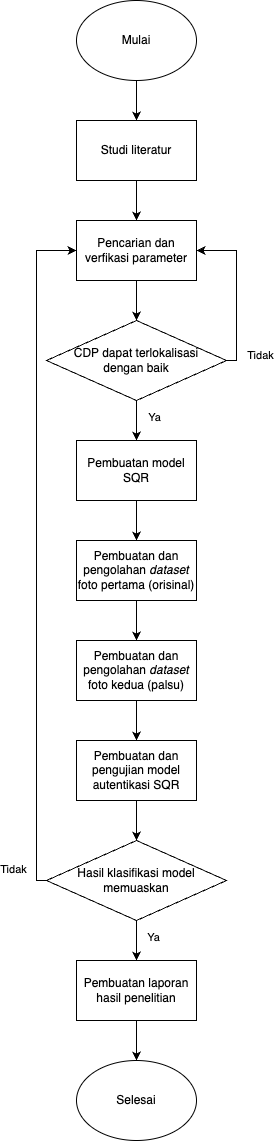
\includegraphics[width=5.5cm]{contents/chapter-3/3-flowchartfix.png}
	\caption{Diagram alir tahapan penelitian}
	\label{Fig: 3-diagramalirpenelitian}
\end{figure}

\clearpage

\section{Pembuatan Model SQR}
\subsection{Penentuan Ukuran dan Versi Kode QR}
Dalam penelitian ini, versi kode QR yang digunakan oleh penulis adalah versi 3. Hal tersebut berdasarkan kebutuhan data yang akan digunakan dalam pembuatan
dataset tidak lebih dari 35 karakter alfanumerik, sehingga kode QR versi 3 dengan ukuran modul 29x29 dapat memenuhi kebutuhan tersebut. Selain itu, adapun
parameter \emph{box-size} dan \emph{border}, yaitu jumlah piksel dari tiap-tiap modul pada kode QR dan lapisan pembatas di luar kode QR. Pada pembuatan model
SQR ini, penulis menetapkan ukuran \emph{box-size} 20 piksel, dan ukuran \emph{border} 3. Setelah itu penulis menambahkan \emph{padding} tambahan berukuran 10
piksel di sisi terluar. Dengan demikian, ukuran total dari SQR adalah (29 x 20) + (2 x (3 x 20)) + (2 x 10) = 720 x 720 piksel.

\subsection{Penentuan Level Toleransi Kerusakan Kode QR}
Dalam pembuatan SQR, nantinya CDP akan ditempelkan atau diletakkan di tengah kode QR. Oleh karena itu, dibutuhkan level toleransi kerusakan yang besar.
Diketahui bahwa level toleransi kerusakan tertinggi yang ada pada kode QR adalah level H dengan toleransi kerusakan kurang lebih 30\%. Oleh karena itu, level
toleransi kerusakan yang dipilih dalam model SQR ini adalah level H.

\subsection{Penentuan Ukuran \emph{Watermark}}
Dengan level toleransi kode QR yang ditentukan adalah level H yang mana menoleransi kurang lebih 30\% kerusakan kode QR, maka ukuran piksel yang dapat dirusak adalah 0,3 x 29 = 8,7. Karena hasilnya tidak bulat, penulis melakukan pembulatan ke atas, sehingga ukuran piksel yang dapat dirusak adalah 9 piksel. Setelah dikalikan dengan \emph{box-size}, maka toleransi kerusakan untuk meletakkan \emph{watermark} adalah 9 x 20 = 180 x 180 piksel.

\subsection{Pembuatan CDP}
Setelah menentukan ukuran \emph{watermark}, selanjutnya adalah mendesain CDP yang digunakan sebagai komponen autentikasi SQR. Dari hasil studi literatur
penulis pada penelitian sebelumnya, CDP yang dinilai efektif adalah berukuran 100x100 piksel \cite{PICARDCANCOPYDETECTIONPATTERN}. Semakin besar ukuran CDP,
pola unit terkecilnya akan menjadi semakin besar. Hal ini menyebabkan informasi yang ada pada CDP tidak terdegradasi maksimal akibat proses P\&S. Ukuran CDP
100x100 piksel dinilai optimal karena tetap sulit untuk dibuat ulang, namun ukuran unit terkecilnya masih kecil.

Penulis di sini akan menggunakan CDP dengan 2 dan 4 level yang nantinya akan dianalisis hasilnya. CDP di-\emph{generate} berdasarkan DATA + SECRET. Hal ini
merupakan salah satu standar keamanan yang banyak digunakan saat ini, menggunakan kombinasi DATA + SECRET yang di-\emph{hash} dan menghasilkan sebuah
\emph{unique identifier}. DATA merupakan nilai data yang tersimpan dalam kode QR, sedangkan SECRET merupakan \emph{string} rahasia yang disimpan oleh
pengembang SQR. DATA + SECRET akan di-\emph{hash} menggunakan algoritma SHA1, kemudan keluarannya diset menjadi heksadesimal. Kemudian batasan nilainya diset
menjadi UINT32 atau memiliki rentang nilai 0 s.d. 4294967296.

Setelah \emph{seed} dibuat yang merupakan keluaran dari fungsi sebelumnya, selanjutnya adalah membuat CDP berukuran 100 x 100 piksel dengan 2 dan 4 level
\emph{grayscale}. Untuk 2 level, nilai \emph{grayscale}-nya adalah [0, 255] dan untuk 4 level, nilai \emph{grayscale}-nya adalah [0, 85, 170, 255]. Nilai-nilai
tersebut didefinisikan secara otomatis hanya dengan memasukkan nilai parameter \emph{quant} saja. Kemudian, untuk memastikan tiap-tiap nilai memiliki
distribusi yang seimbang dalam CDP, penulis membatasi perbandingan distribusi maksimal antar nilai adalah 1:3, misal untuk 4 level perbandingan distribusi yang
dapat dipilih adalah [[1, 1, 1, 1], [3, 1, 2, 1], …, [1, 1, 3, 1]]. Program nantinya akan memilih secara acak dari 10 variasi distribusi yang ada. Kemudian
barulah CDP berukuran 100 x 100 piksel di-\emph{generate} secara acak berdasarkan nilai \emph{seed}, sehingga nilai \emph{seed} akan berpengaruh pada
distribusi elemen dan letak tiap-tiap elemen dalam CDP.

\subsection{Menentukan Jumlah, Jenis, Letak, dan Ukuran Penanda ArUco}
Setelah CDP dibuat, ruang kosong yang tersisa di dalam \emph{watermark} adalah 180 - 100 = 80 piksel. Sisa ruang kosong tersebut digunakan untuk meletakkan
penanda ArUco sebagai pembantu dalam melokalisasi objek CDP yang akan digunakan untuk autentikasi SQR. Jumlah penanda ArUco yang digunakan adalah 8 buah.
Kedelapan penanda ArUco diletakkan di area kosong di sekitar CDP, pojok kiri atas, tengah atas, pojok kanan atas, kiri tengah, kanan tengah, pojok kiri bawah,
tengah bawah, dan pojok kanan bawah. Kedelapan penanda tersebut dinilai penulis cukup untuk merepresentasikan dan mewakili titik-titik yang nantinya akan
digunakan untuk transformasi homografi. Penelitian sebelumnya menggunakan empat titik, yaitu keempat titik sudut kode QR. Hal tersebut memiliki kelemahan,
yaitu jika ada \emph{bending} pada foto pada bagian sisi-sisi kode QR (misal kode QR ditempelkan pada permukaan tabung), maka hasil transformasi homografinya
akan kurang maksimal. Selanjutnya, untuk memudahkan program dalam mendeteksi kedelapan penanda ArUco, maka tentunya pola ArUco yang paling sederhana dapat
memudahkan program dalam pendeteksian. Oleh karena itu, penulis memilih ArUco dengan ukuran modul 4 piksel. Pada Gambar \ref{Fig: 3-aruco4x4} dan Gambar
\ref{Fig: 3-aruco6x6} dapat dilihat bahwa ArUco dengan ukuran modul 4 piksel memiliki pola yang relatif sederhana, sehingga toleransi degradasi gambar akibat
proses P\&S dapat diminimalisir.

\begin{figure}[!ht]
	\centering
	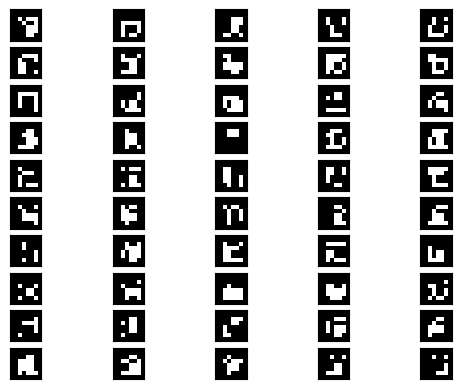
\includegraphics[width=7cm]{contents/chapter-3/3-aruco4x4.png}
	\caption{Sampel 50 penanda ArUco dengan ukuran modul 4x4 piksel}
	\label{Fig: 3-aruco4x4}
\end{figure}

\begin{figure}[!ht]
	\centering
	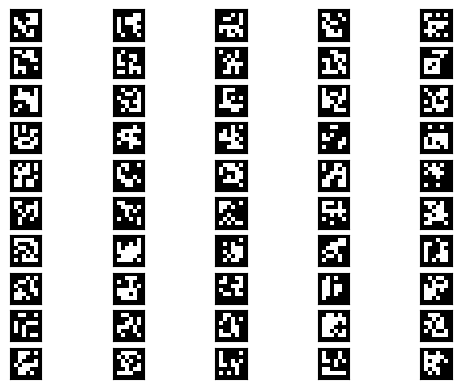
\includegraphics[width=7cm]{contents/chapter-3/3-aruco6x6.png}
	\caption{Sampel 50 penanda ArUco dengan ukuran modul 6x6 piksel}
	\label{Fig: 3-aruco6x6}
\end{figure}

Terakhir, adalah menentukan ukuran penanda ArUco yang diletakkan di sekitar CDP. Metode yang digunakan untuk mendapatkan ukuran adalah dengan membuat
\emph{dataset} sebanyak 40 data yang tiap 5 datanya memiliki ukuran ArUco 20 s.d. 34 piksel. Kemudian nantinya akan diuji, penanda ArUco dengan ukuran
berapakah yang memiliki akurasi lokalisasi paling tinggi yang berarti kedelapan penanda ArUco dapat terdeteksi oleh program. Tiap-tiap penanda ArUco memiliki
id unik yang membedakan penanda satu dengan lainnya dalam sebuah pustaka penanda ArUco. Oleh karena itu, penulis menggunakan id penanda ArUco tetap, yaitu 0
s.d. 7 untuk memudahkan pemetaan titik asal ke titik tujuan saat melakukan transformasi homografi, misalnya titik tujuan pojok kiri atas harus ditempati oleh
penanda ArUco dengan id = 0, titik pojok kanan bawah harus ditempati oleh marker dengan id = 7 dan seterusnya.

\subsection{Menempelkan \emph{Watermark} ke SQR} Setelah seluruh komponen \emph{watermark} berukuran 180 x 180 piksel selesai dibuat, selanjutnya adalah menempelkannya atau meletakkannya ke
tengah-tengah kode QR yang telah dibuat di awal. Hal ini dapat dilakukan dengan menggunakan fitur \emph{slicing} pada NumPy \emph{array}.

\section{Pembuatan dan Pengolahan \emph{Dataset} SQR Foto Pertama (Orisinal)}
\subsection{Pembuatan \emph{Batch} SQR Foto Pertama (Orisinal)} \label{Pembuatan Batch SQR Foto Pertama (Orisinal)} SQR berjumlah 40 akan disusun menjadi 1 \emph{batch}, dengan konfigurasi 8
baris 5 kolom. Diketahui juga bahwa ukuran satu SQR yang telah dirancang adalah 720 x 720 piksel. Nantinya SQR akan dirancang untuk dicetak dengan ukuran 55 x
55 mm, sehingga jumlah piksel per milimeter pada batch QR adalah 720 / 55 = 13 ppmm (piksel per milimeter). Kemudian, untuk menyesuaikan ukuran piksel terhadap
milimeter, perlu dilakukan penskalaan terhadap ppmm serta pemberian \emph{padding}. Diketahui ukuran kertas A3+ adalah 329 x 483 mm, jika dijadikan ukuran
piksel dengan 13 ppmm, maka ukurannya menjadi 4307 x 6323 piksel. Kemudian \emph{padding} horizontal diset sebesar (6323 - (720 x 55)) / 2 = 281,5 sedangkan
\emph{padding} vertikal diset sebesar (4307 - (72 0x 8) / 2 = 353,5. Karena hasilnya tidak bulat, maka \emph{padding} horizontal dan vertikalnya diset ke +-
bilangan bulat terdekat. Hasil akhir \emph{batch} dalam ukuran piksel dapat dilihat pada Gambar \ref{Fig: 3-batchqr}.

\begin{figure}[!ht]
	\centering
	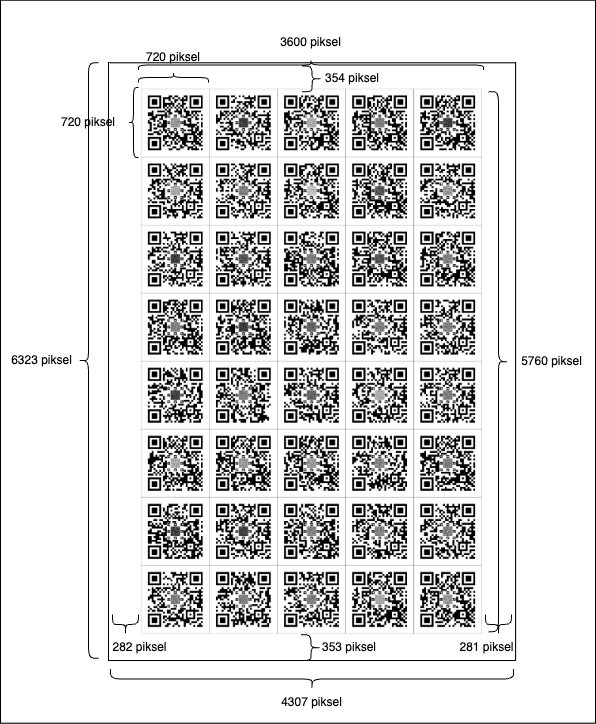
\includegraphics[width=10cm]{contents/chapter-3/3-batchqr.png}
	\caption{\emph{Batch} SQR orisinal (foto pertama) dalam ukuran piksel}
	\label{Fig: 3-batchqr}
\end{figure}

\subsection{Pencetakan \emph{Batch} SQR Foto Pertama (Orisinal)} \label{Pencetakan Batch SQR Foto Pertama (Orisinal)} Dari hasil \emph{generate batch} oleh program yang berukuran piksel dan
berformat PNG, hasil tersebut masih perlu di-\emph{scaling} menjadi ukuran kertas A3+ dengan format PDF, sesuai dengan standar percetakan. Untuk melakukannya,
penulis menggunakan perangkat lunak tambahan, yaitu Adobe Photoshop. Caranya adalah meng-\emph{import} \emph{batch} PNG ke dalam Photoshop, kemudian tekan CTRL
+ P untuk melakukan pencetakan. Kemudian di panel konfigurasi pencetakan, centang bagian \emph{Scale to Fit Media}, hal ini bertujuan untuk melakukan
penskalaan menuju ukuran kertas yang dituju. Selanjutnya, jika belum ada, masukkan konfigurasi untuk ukuran kertas A3+, yaitu dengan ukuran 329 x 483 mm.
Terakhir adalah ubah target cetak menjadi PDF. Langkah-langkah lengkap konfigurasi pencetakan dan ukuran kertas dapat dilihat pada Gambar \ref{Fig:
	3-konfigurasips1} dan Gambar \ref{Fig: 3-konfigurasips2}.

\begin{figure}[!h]
	\centering
	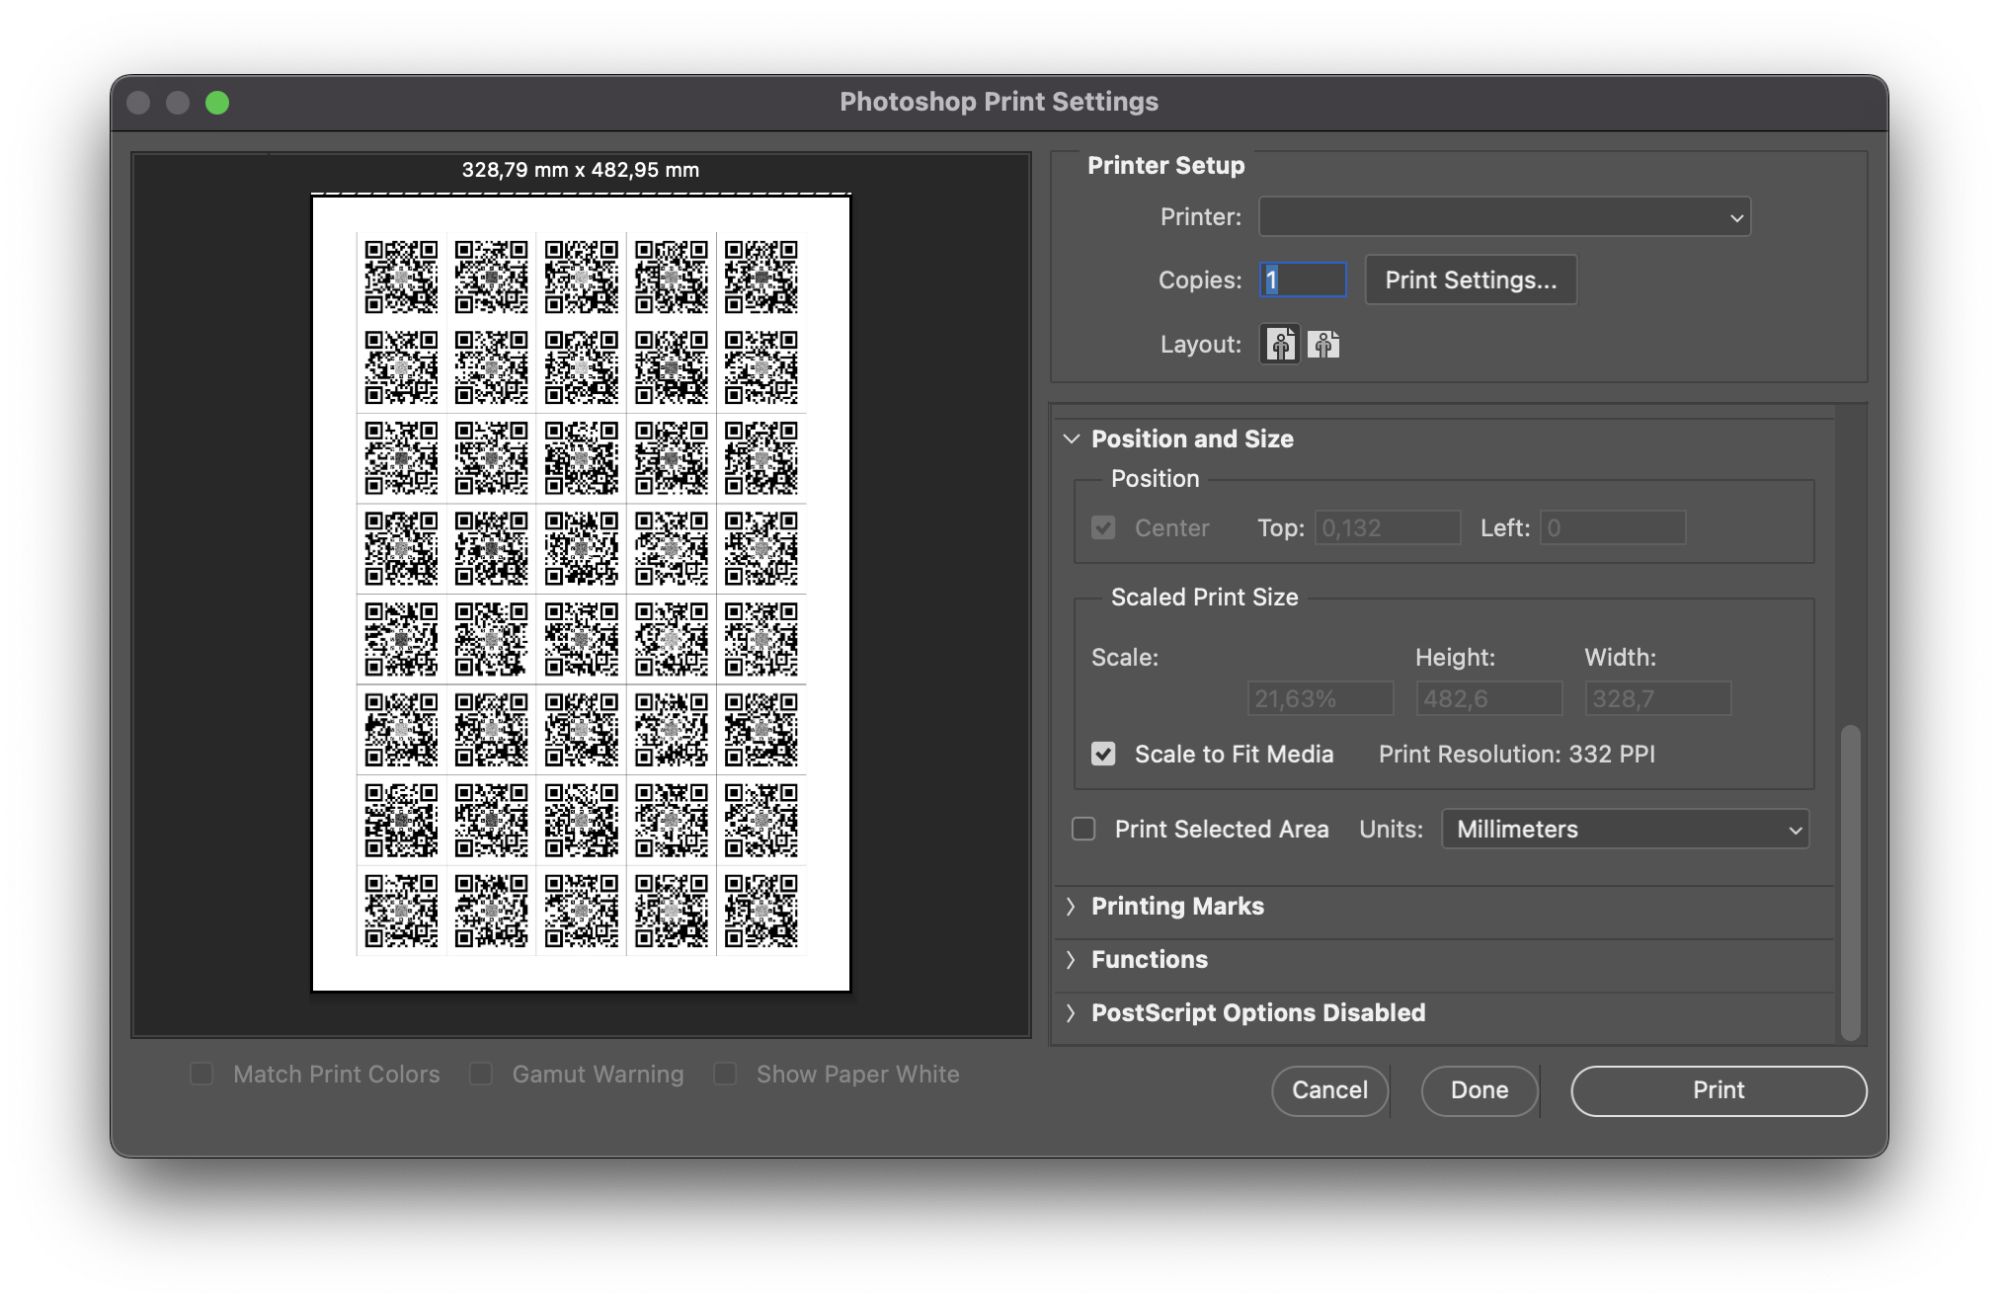
\includegraphics[width=8cm]{contents/chapter-3/3-konfigurasips1.png}
	\caption{Konfigurasi saat melakukan pencetakan menggunakan Adobe Photoshop}
	\label{Fig: 3-konfigurasips1}
\end{figure}

\begin{figure}[!h]
	\centering
	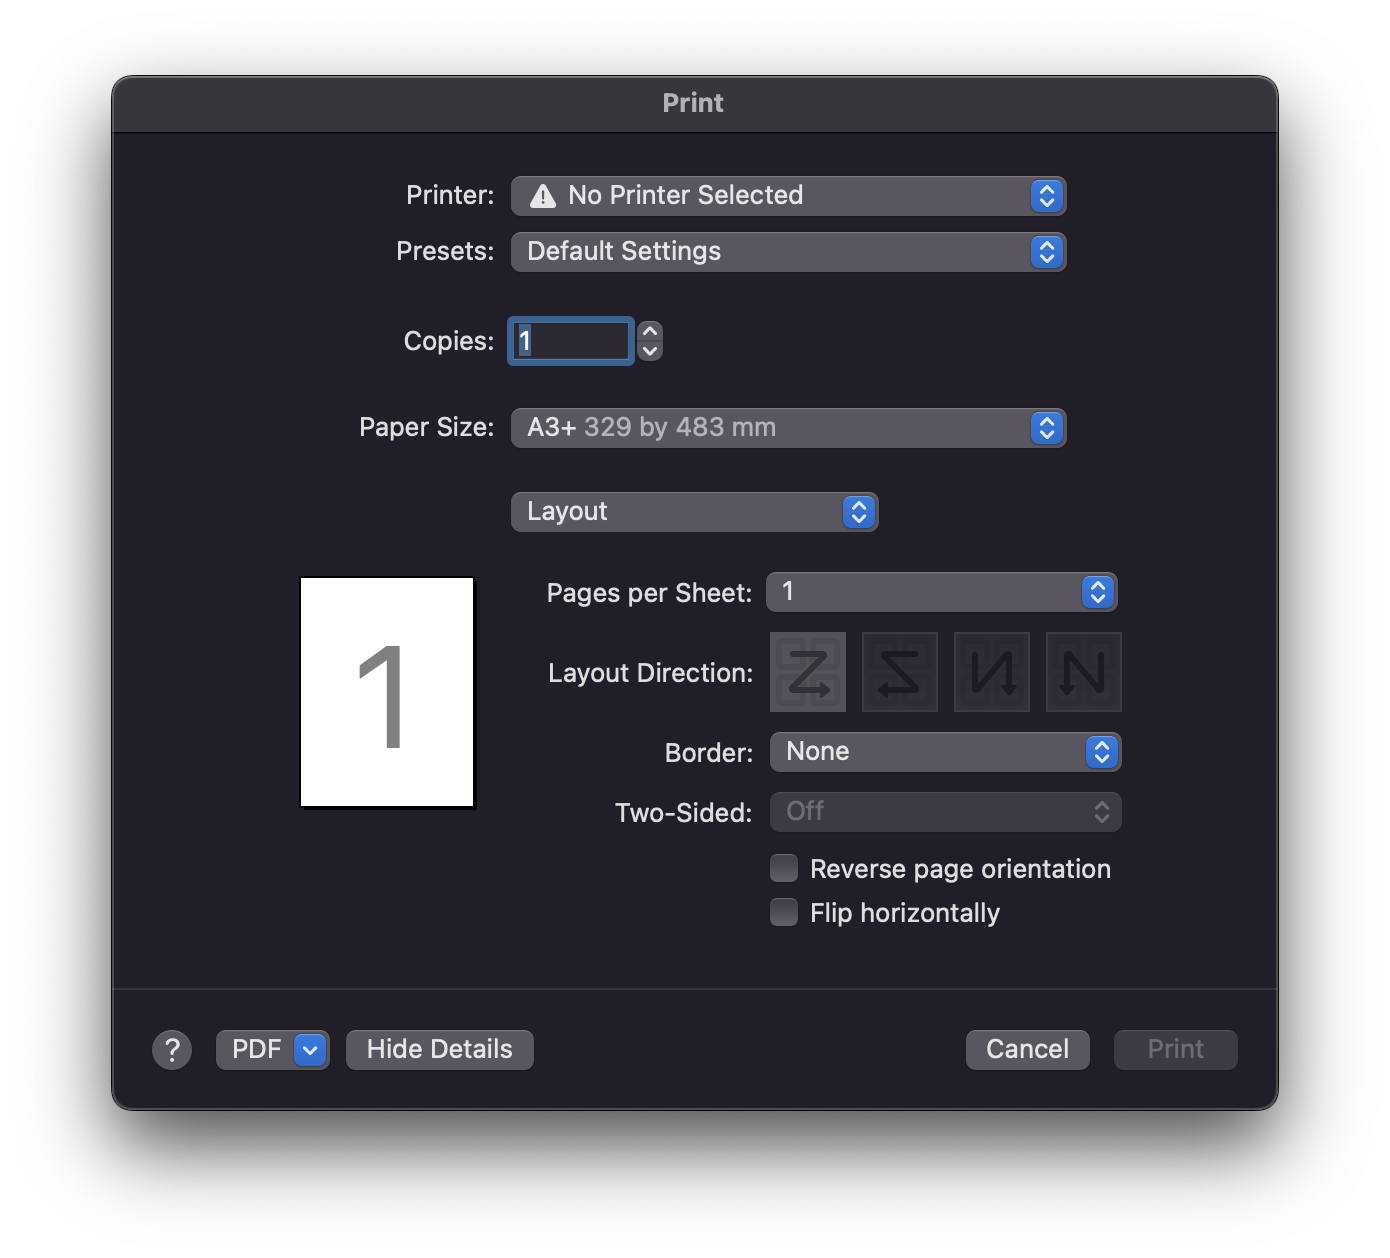
\includegraphics[width=8cm]{contents/chapter-3/3-konfigurasips2.png}
	\caption{Konfigurasi menambahkan ukuran kertas A3+ dan cetak menjadi PDF}
	\label{Fig: 3-konfigurasips2}
\end{figure}

\noindent Terakhir, untuk jenis kertas dan tinta yang digunakan haruslah bersifat \emph{doff}. Hal ini supaya hasil pemotretan tidak memantulkan cahaya ketika dipotret menggunakan flash dari kamera.

\subsection{Pemotretan \emph{Dataset} SQR Foto Pertama (Orisinal)} \label{Pemotretan Dataset SQR Foto Pertama (Orisinal)} Pemotretan \emph{dataset} foto pertama (orisinal) dilakukan menggunakan
boks. Boks dibuat dengan kardus yang dilubangi bagian depan dan atasnya, kemudian sisi dalamnya ditempeli kertas putih supaya dapat menghasilkan hasil
pemotretan yang terang. Penggunaan boks dalam pemotretan \emph{dataset} dapat menjaga kualitas \emph{dataset} dan juga meningkatkan kecepatan pengambilan
\emph{dataset}. Pemotret hanya perlu mengganti SQR tanpa harus memindah-mindahkan \emph{smartphone} yang digunakan untuk memotret. Lingkungan pemotretan
menggunakan boks yang penulis gunakan dalam mendapatkan \emph{dataset} orisinal dapat dilihat pada Gambar \ref{Fig: 3-lingkunganpemotretan}.

\begin{figure}[!h]
	\centering
	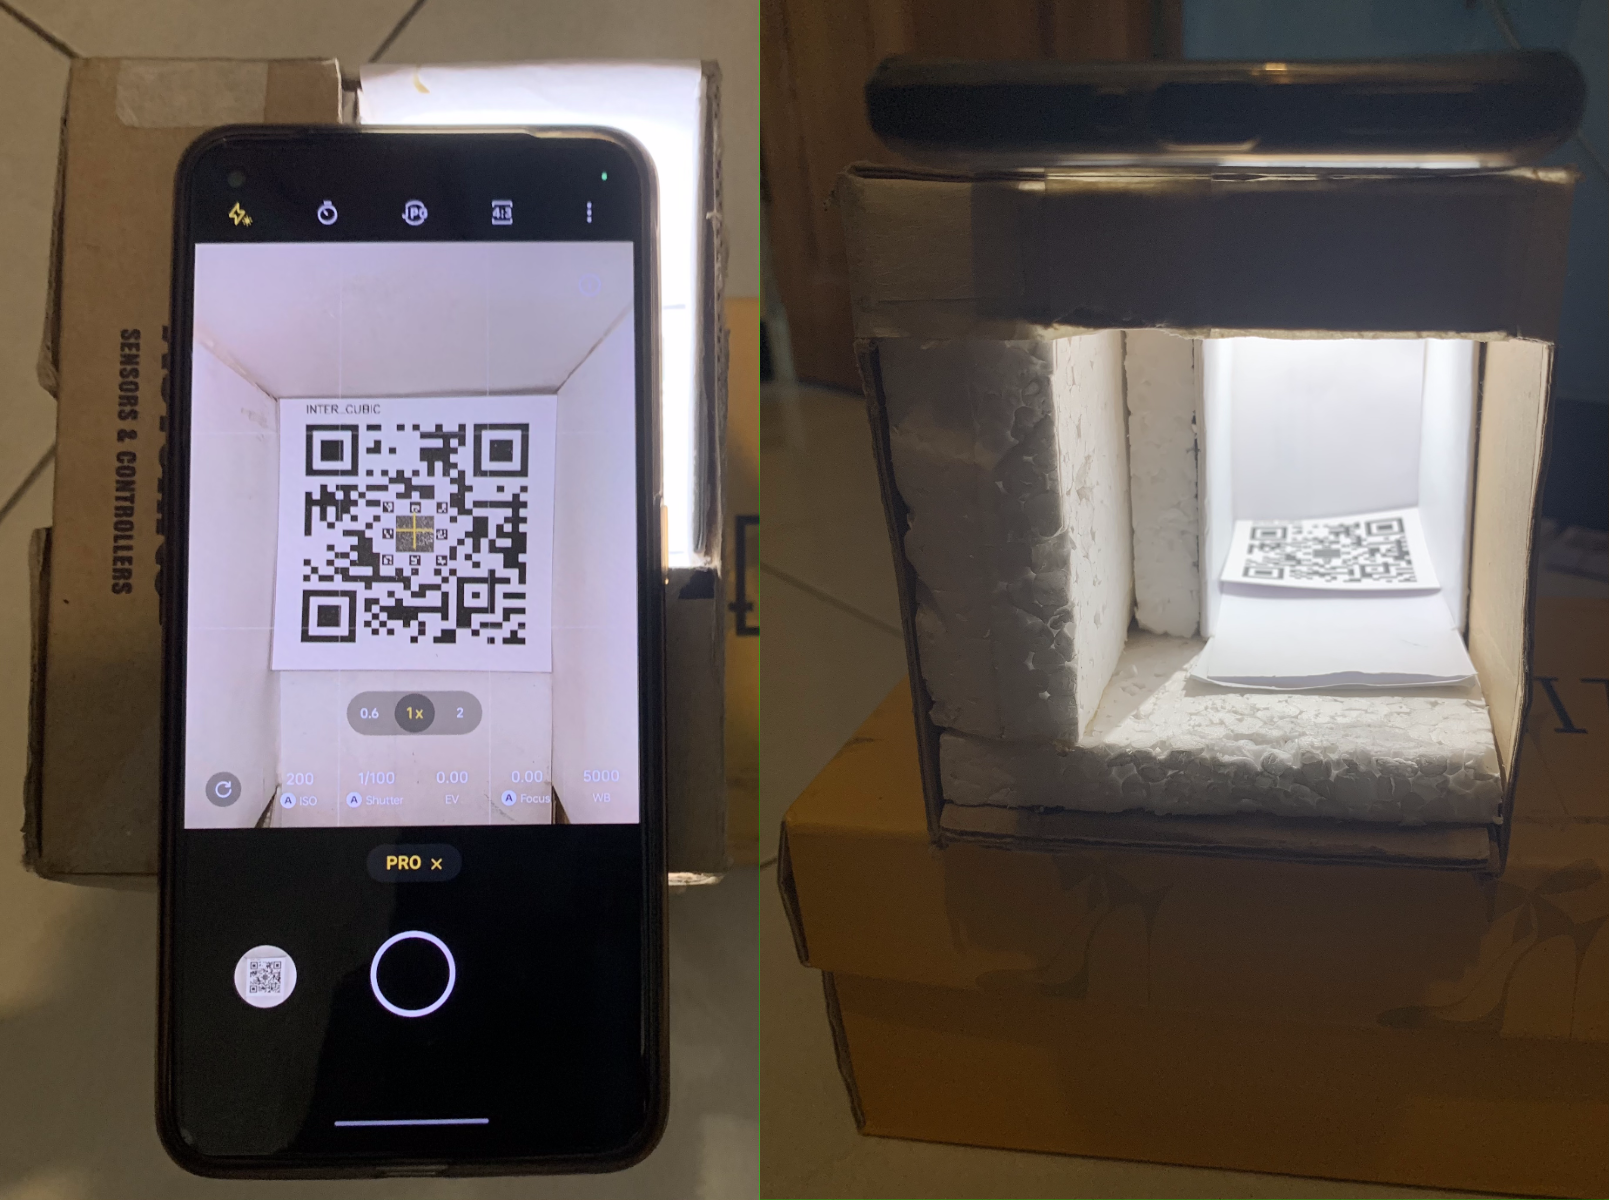
\includegraphics[width=8cm]{contents/chapter-3/3-environmentpemotretan.png}
	\caption{Lingkungan pemotretan menggunakan boks untuk melakukan pemotretan \emph{dataset} SQR}
	\label{Fig: 3-lingkunganpemotretan}
\end{figure}

\subsection{Lokalisasi CDP dari \emph{Raw} Foto Pertama (Orisinal)} \label{Lokalisasi CDP dari Raw Foto Pertama (Orisinal)}
\subsubsection{Mengganti Nama Fail}
Untuk melakukan lokalisasi CDP dari \emph{dataset} foto, langkah pertama yang dilakukan adalah mengganti nama fail foto sesuai dengan data yang ada dalam kode
QR. Hal ini bertujuan untuk memudahkan pengelolaan \emph{dataset}. Nama fail sebelum dan sesudah perubahan nama dapat dilihat pada Gambar \ref{Fig:
	3-namafile1} dan Gambar \ref{Fig: 3-namafile2}.

\begin{figure}[h]
	\centering
	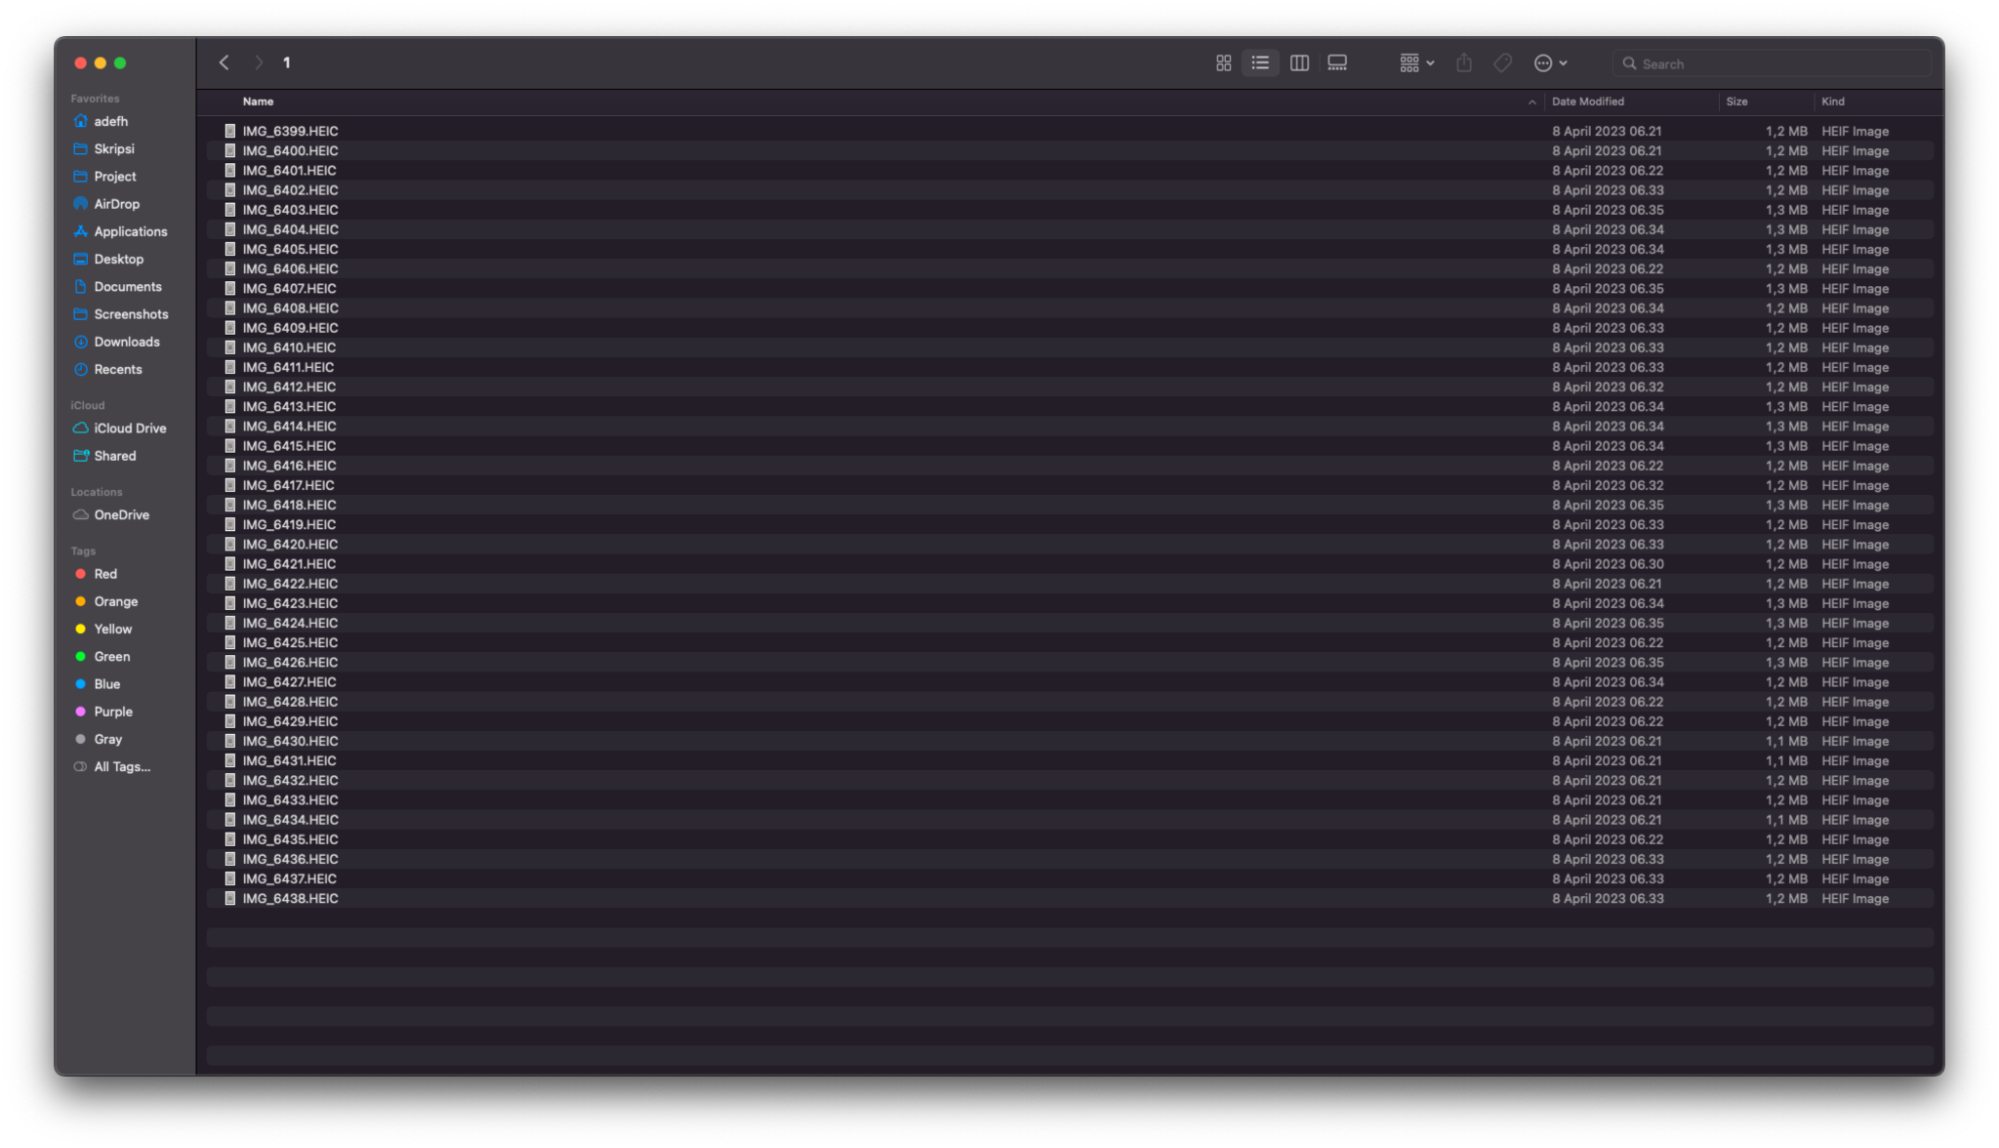
\includegraphics[width=10cm]{contents/chapter-3/3-namafile1.png}
	\caption{Nama fail sebelum perubahan}
	\label{Fig: 3-namafile1}
\end{figure}

\begin{figure}[h]
	\centering
	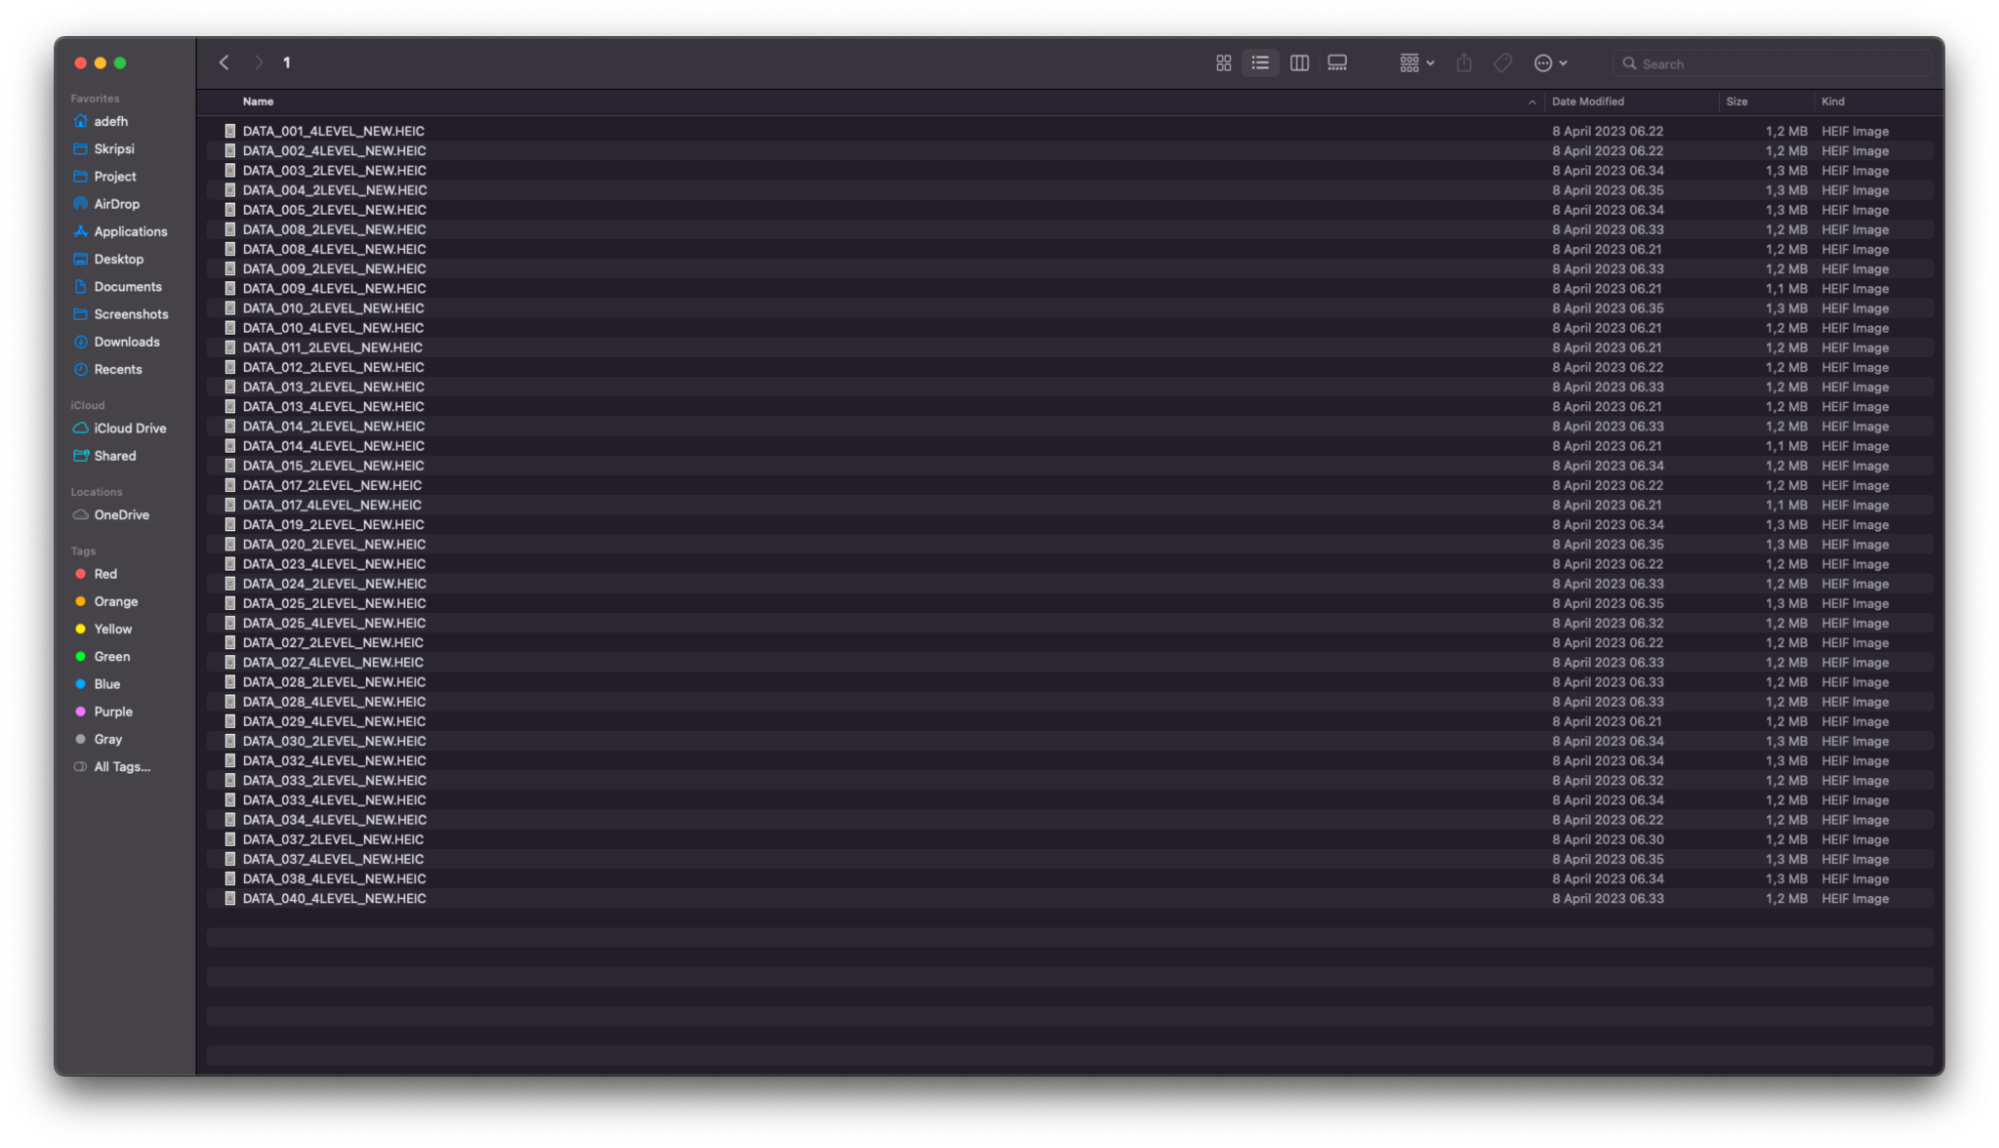
\includegraphics[width=10cm]{contents/chapter-3/3-namafile2.png}
	\caption{Nama fail setelah perubahan}
	\label{Fig: 3-namafile2}
\end{figure}

Untuk mengganti nama fail, penulis memanfaatkan pustaka OpenCV yang digunakan untuk mendeteksi data dalam kode QR. Pustaka tersebut juga dapat digunakan untuk
mendeteksi koordinat keempat titik sudut kode QR yang digunakan dalam penelitian sebelumnya untuk melakukan transformasi homografi dari titik asal ke titik
tujuan. Sebelum dideteksi dan di-\emph{decode} gambar foto \emph{raw} akan diproses terlebih dahulu, untuk meningkatkan performa deteksi oleh pustaka
QRDecoder. Pemrosesan yang dilakukan yaitu, mengubah gambar menjadi \emph{grayscale} dan menambahkan filter GaussianBlur pada gambar yang telah diubah menjadi
\emph{grayscale} dengan ukuran kernel tertentu. Hal ini bertujuan untuk menghilangkan derau dari gambar. Setelah itu, akan dilakukan perulangan \emph{scaling}
pada gambar dengan faktor skala 1 s.d. 0,1. Pada tiap-tiap faktor skala, fungsi QRDecoder akan mencoba mendeteksi keempat titik sudut kode QR dan data di
dalamnya. Jika titik sudut yang dideteksi sudah berjumlah 4 dan data di dalamnya sudah terdeteksi, maka proses penskalaan akan dihentikan pada faktor skala
tertinggi, lalu kemudian data yang tersimpan pada kode QR akan dikeluarkan. Misal, saat perulangan dengan faktor skala 1, empat titik sudut pada kode QR sudah
terdeteksi dan datanya juga, jika hasilnya demikian, artinya gambar tidak perlu di-\emph{scaling} lagi. Namun, apabila perulangan berhenti di faktor skala 0,5,
artinya gambar perlu di-\emph{scaling} setengahnya untuk dapat dideteksi dan di-\emph{decode} datanya.

\subsubsection{Lokalisasi CDP dari Foto}
Untuk melakukan lokalisasi CDP dari foto yang telah diganti nama fail-nya, penulis memanfaatkan penanda ArUco yang diletakkan di sekitar CDP. Telah dijelaskan
sebelumnya, bahwa delapan penanda ArUco dapat melakukan lokalisasi CDP dengan lebih baik karena titik yang digunakan untuk transformasi homografi dari titik
asal ke titik tujuan lebih banyak dari empat titik yang didapatkan dari fungsi QRDecoder. Hal ini dapat mengatasi masalah \emph{bending} gambar pada kondisi
tertentu. Sama seperti pemrosesan sebelumnya, gambar akan diubah menjadi \emph{grayscale} dan ditambahkan filter GaussianBlur untuk meningkatkan performa
deteksi penanda ArUco. Kemudian, gambar akan dilakukan perulangan penskalaan dengan faktor skala 1 s.d. 0,1. Pada tiap-tiap faktor skala, fungsi
aruco.detectMarkers akan mendeteksi titik-titik sudut dari kedelapan penanda ArUco beserta id-nya. Sama seperti pendeteksian data pada kode QR, perulangan akan
dihentikan apabila delapan penanda ArUco sudah berhasil dideteksi.

Dari keluaran empat titik sudut di tiap-tiap penanda, penulis memrosesnya untuk menjadikannya satu titik di tengah untuk memudahkan pendefinisian titik asal
transformasi. Kemudian hasilnya akan diolah menjadi xy\_list, yaitu koordinat titik tengah dari masing-masing penanda mulai dari id = 0 s.d. id = 7. Contoh
xy\_list yang telah diolah dapat dilihat pada Gambar \ref{Fig: 3-xylist}.

\begin{figure}[h]
	\centering
	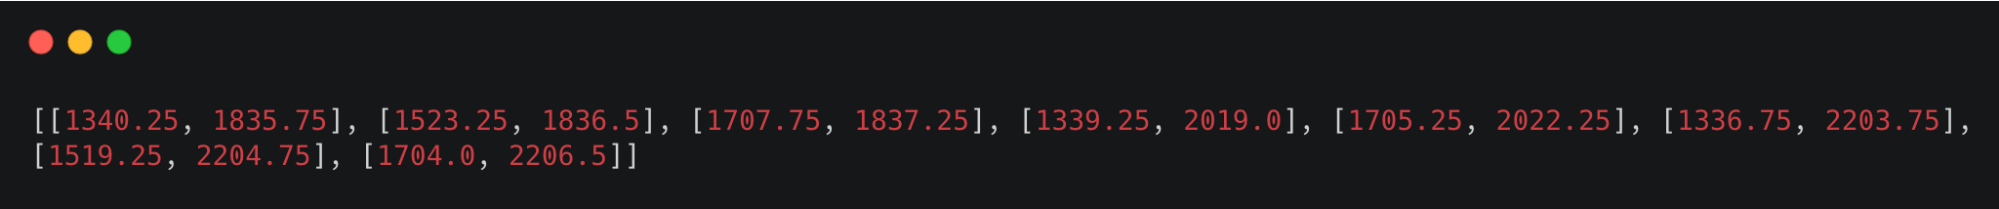
\includegraphics[width=13cm]{contents/chapter-3/3-xylist.png}
	\caption{xy\_list yang menyimpan koordinat titik tengah penanda ArUco dari id 0 s.d. 7}
	\label{Fig: 3-xylist}
\end{figure}

\noindent Untuk contoh plot hasil deteksi koordinat ke dalam xy\_list pada gambar hasil foto dapat dilihat pada Gambar \ref{Fig: 3-plotxylist}.

\begin{figure}[h]
	\centering
	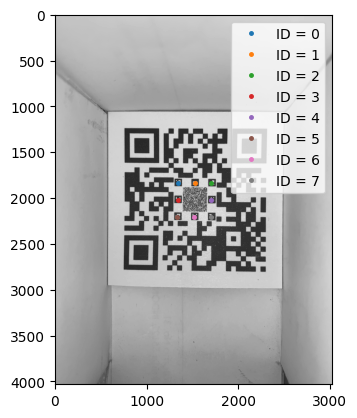
\includegraphics[width=8cm]{contents/chapter-3/3-plotxylist.png}
	\caption{Hasil plot koordinat titik tengah penanda ArUco pada xy\_list ke gambar hasil foto}
	\label{Fig: 3-plotxylist}
\end{figure}

Setelah semua titik telah didapatkan, selanjutnya adalah melakukan transformasi homografi dari kedelapan titik tersebut ke titik tujuan. Untuk menentukan titik
tujuan, penulis menggunakan acuan ukuran dari jarak terdekat dari empat titik penanda ArUco yang terletak di pojok (pojok kiri atas, pojok kanan atas, pojok
kiri bawah, dan pojok kanan bawah) atau (id 0, id 2, id 5, dan id 7) menggunakan \emph{euclidean distance}. Hal ini digunakan untuk menjaga kualitas hasil dari
transformasi homografi. Dari eksperimen, jika ukuran tujuan transformasi homografi terlalu jauh dari ukuran awal, misalnya langsung didefinisikan berukuran 100
x 100 piksel sesuai \emph{template} hasilnya akan rusak. Setelah jarak terdekatnya didapatkan sebagai x, selanjutnya adalah menentukan titik tujuan. Titik
tujuan transformasi didefinisikan dalam bentuk sebuah \emph{list} seperti yang terlihat pada Gambar \ref{Fig: 3-koordinattujuan}, dimana x merupakan jarak
terdekat dari penanda ArUco yang terletak di pojok.

\begin{figure}[h]
	\centering
	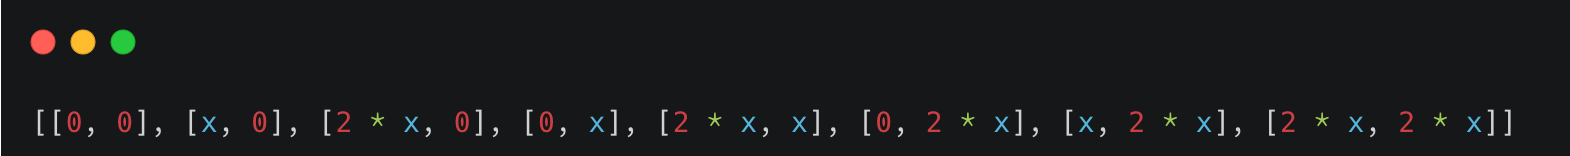
\includegraphics[width=13cm]{contents/chapter-3/3-koordinattujuan.png}
	\caption{\emph{List} koordinat tujuan transformasi homografi}
	\label{Fig: 3-koordinattujuan}
\end{figure}

Dalam melakukan transformasi homografi, koordinat tujuan nilainya dikalikan dengan 2, sehingga ukuran dari CDP terlokalisasi adalah 2 kali dari CDP awal
sebelum dilokalisasi. Hal ini bertujuan untuk menjaga kualitas CDP yang nantinya masih akan diproses lagi. Untuk melihat perbedaan SQR awal dan SQR setelah
ditransformasi homografi berdasarkan koordinat dari penanda ArUco dapat dilihat pada Gambar \ref{Fig: 3-hasillokalisasi}.

\begin{figure}[h]
	\centering
	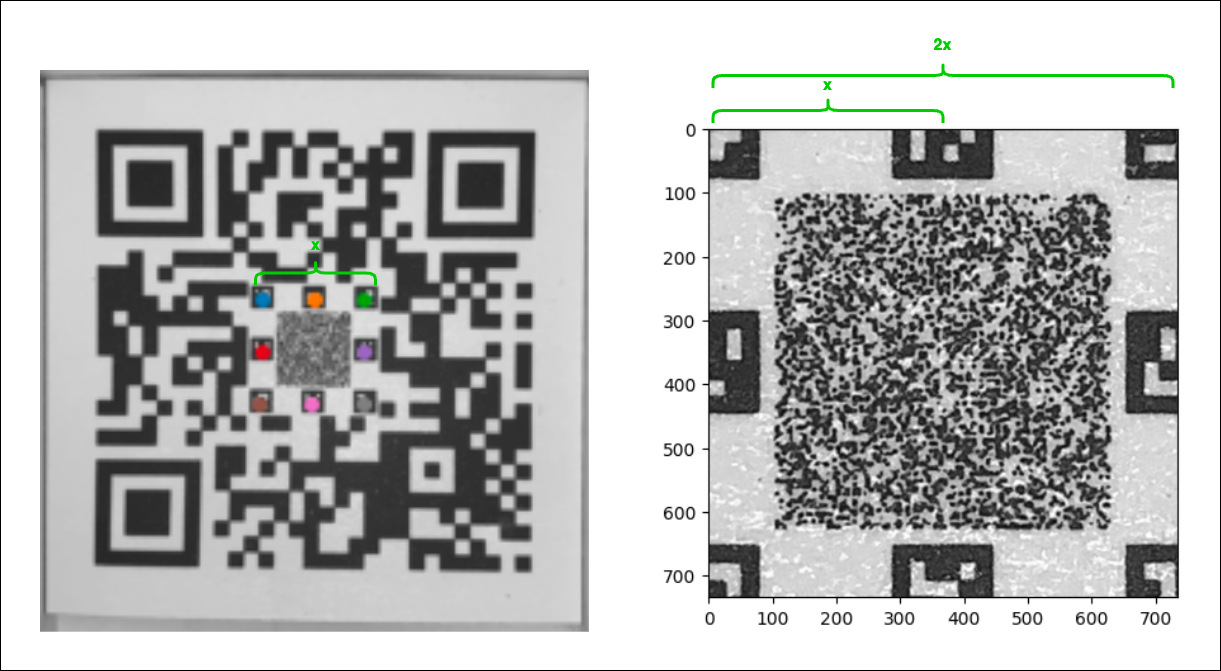
\includegraphics[width=10cm]{contents/chapter-3/3-hasillokalisasi.png}
	\caption{SQR awal dan setelah dilakukan transformasi homografi}
	\label{Fig: 3-hasillokalisasi}
\end{figure}

Setelah melakukan transformasi homografi, langkah selanjutnya adalah mendapatkan objek CDP itu sendiri. Diketahui bahwa desain pada desain SQR awal, CDP
berukuran 100 x 100 piksel, sedangkan ukuran gambar \emph{watermark} hingga titik tengah penanda ArUco adalah 140x140 piksel. Oleh karena itu, untuk
mendapatkan objek CDP dari objek hasil transformasi adalah dengan melakukan pemotongan di tengah sebesar 100/140 bagian dari objek hasil transformasi. Setelah
objek CDP didapatkan, langkah terakhir adalah melakukan penskalaan CDP menjadi 100 x 100 piksel sesuai dengan ukuran \emph{template}. CDP hasil lokalisasi
berukuran 100 x 100 piksel inilah yang akan diolah datanya untuk dibandingkan dengan \emph{template}. Perbandingan CDP \emph{template} dengan CDP hasil akhir
dari lokalisasi dapat dilihat pada Gambar \ref{Fig: 3-templatevslokalisasi}. Kemudian untuk memudahkan manajemen fail CDP sebagai \emph{dataset}, hasil
lokalisasi disimpan menjadi sebuah fail gambar berformat PNG dengan format penamaan fail CDP\_\{data\}.png. Hasil akhir dataset CDP foto pertama (orisinal)
dikumpulkan ke dalam sebuah folder seperti pada Gambar \ref{Fig: 3-hasildatasetcdp}.

\begin{figure}[h]
	\centering
	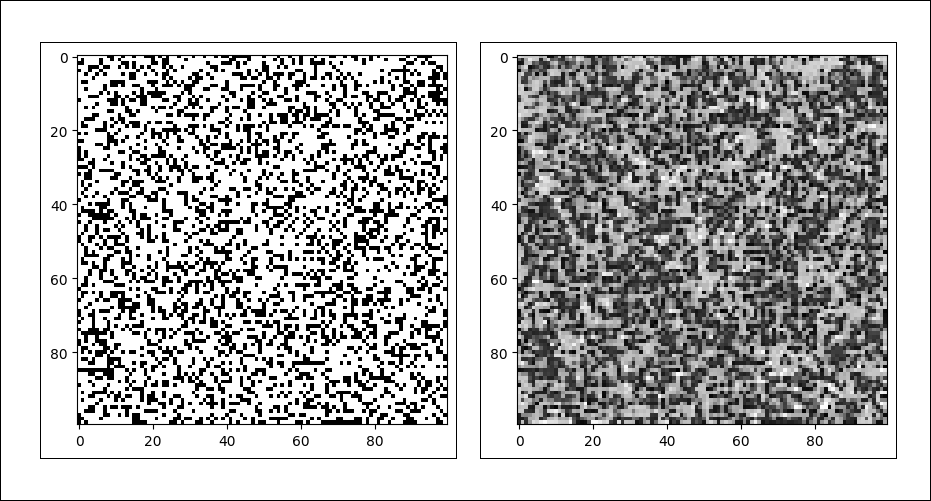
\includegraphics[width=10cm]{contents/chapter-3/3-templatevslokalisasi.png}
	\caption{Perbandingan CDP \emph{template} dengan CDP hasil lokalisasi foto pertama (orisinal)}
	\label{Fig: 3-templatevslokalisasi}
\end{figure}

\begin{figure}[h]
	\centering
	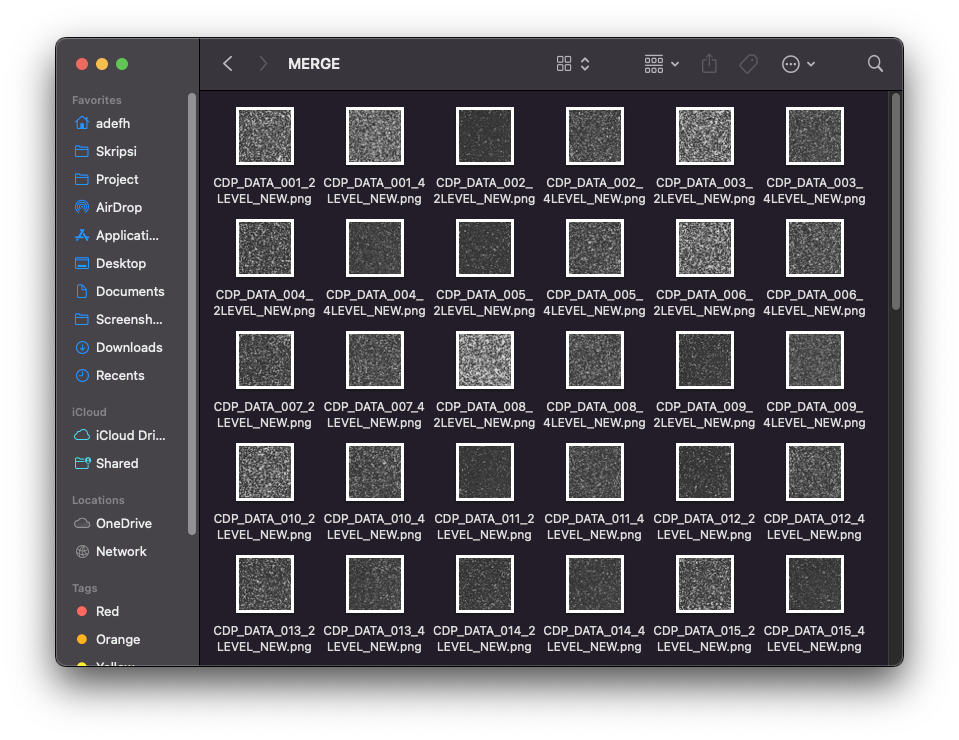
\includegraphics[width=10cm]{contents/chapter-3/3-hasildatasetcdp.png}
	\caption{Hasil \emph{dataset} CDP foto pertama (orisinal) yang sudah dilokalisasi dan diganti nama failnya}
	\label{Fig: 3-hasildatasetcdp}
\end{figure}

\subsection{Pembuatan Fitur Jarak (Orisinal dengan \emph{Template})} \label{Pembuatan Fitur Jarak {Orisinal dengan Template}}
Untuk mendapatkan fitur dari \emph{dataset} foto pertama (orisinal) yang nantinya digunakan dalam pembuatan model klasifikasi menggunakan AutoML, penulis menggunakan jarak spasial, histogram, dan DCT dengan beberapa koefisien jarak dari CDP foto pertama (orisinal) dengan \emph{template}.

Langkah pertama adalah membaca seluruh fail CDP dalam folder yang sudah ditentukan, kemudian dilakukan \emph{parsing} pengambilan jenis interpolasi dan data
sesuai dengan format penamaan \emph{dataset} CDP. Selanjutnya adalah men-\emph{generate} \emph{template} berdasarkan data yang sudah di-\emph{parsing}, simpan
sebagai \emph{template}. Setelah itu, baca CDP hasil scan, ubah menjadi \emph{grayscale}, simpan sebagai \emph{scanned}. Kemudian, tiap fail CDP
\emph{template} dan \emph{scanned} akan diperbesar 4 kali pembesaran, dari awalnya 100 x 100 piksel di-\emph{scaling} menjadi 400 x 400 piksel. Selanjutnya,
matriks tersebut akan diolah menjadi tiga fitur, yaitu DCT, histogram, dan spasial. Kemudian akan dihitung jaraknya menggunakan koefisien jarak korelasi,
kosinus, \emph{euclidean}, dan \emph{canberra} untuk tiap-tiap fitur. Untuk tiap perulangan (tiap pembacaan fail) hasil fitur jarak, data, jenis interpolasi,
dan level (2 atau 4 level) akan di-\emph{append} ke dalam sebuah \emph{list}. Setelah perulangan selesai, \emph{list} tersebut akan diubah menjadi sebuah
\emph{dataframe}, di-\emph{sorting} berdasarkan jenis interpolasi dan datanya, lalu ditambahkan kolom label (orisinal atau palsu). Setelah \emph{dataframe}
siap, selanjutnya adalah mengekspor \emph{dataframe} tersebut menjadi sebuah fail csv. Untuk hasil akhir \emph{dataframe} sebelum diekspor menjadi fail csv
dapat dilihat pada Gambar \ref{Fig: 3-dataframefitur}.

\begin{figure}[h]
	\centering
	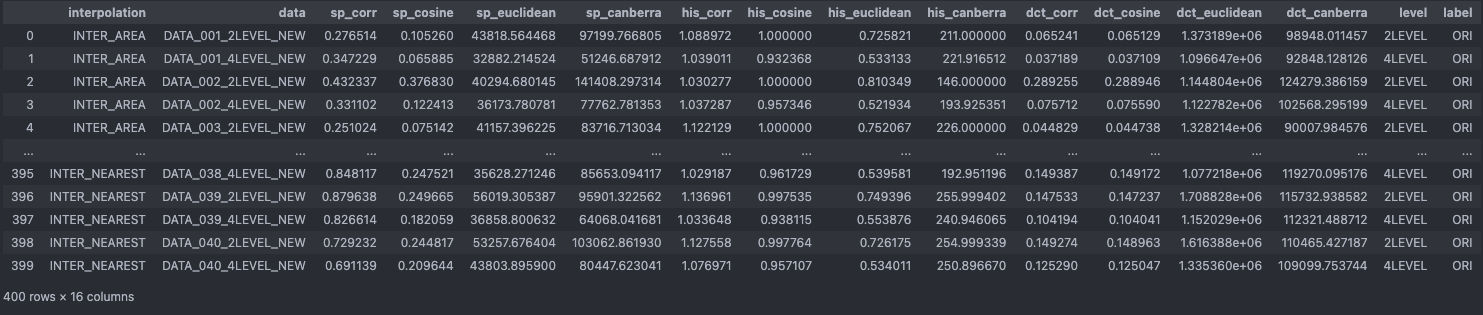
\includegraphics[width=\textwidth]{contents/chapter-3/3-dataframefitur.png}
	\caption{\emph{Dataframe} fitur jarak \emph{dataset} foto pertama (orisinal)}
	\label{Fig: 3-dataframefitur}
\end{figure}

\subsection{Analisis \emph{Dataset} CDP Foto Pertama (Orisinal)} Setelah seluruh \emph{dataset} CDP foto pertama (orisinal) sudah siap, selanjutnya adalah melakukan analisis menggunakan
\emph{dataframe} fitur jarak. Hal pertama yang dianalisis apakah ada perbedaan signifikan antara jarak CDP orisinal dengan \emph{template} untuk CDP 2 dan 4
level. Analisis selanjutnya adalah mengetahui perbedaan rata-rata jarak dari berbagai interpolasi penskalaan yang digunakan untuk melokalisasi CDP. Dari hasil
tersebut, nantinya akan dibuat CDP palsu menggunakan interpolasi penskalaan yang hasil jaraknya paling kecil antara foto pertama (orisinal) dengan
\emph{template}. Hal ini dimaksudkan untuk membuat CDP palsu yang semirip mungkin dengan CDP asli. Uji signifikansi dilakukan menggunakan metode \emph{T-test},
sedangkan untuk mencari rata-rata jarak dari data grup tiap interpolasi penskalaan, penulis menggunakan fitur \emph{describe} yang telah disediakan oleh
pustaka Pandas.

\section{Pembuatan dan Pengolahan \emph{Dataset} SQR Foto Kedua (Palsu)}
\subsection{Pembuatan Model SQR Foto Kedua (Palsu)}
Model SQR palsu dibuat dengan men-\emph{generate} \emph{template} sesuai data pada SQR orisinal. Kemudian CDP hasil lokalisasi foto pertama akan ditempelkan di
tengah-tengah \emph{template} SQR, sehingga perbedaan antara SQR orisinal dan palsu hanya ada pada CDP-nya saja. Hal ini tentu akan sulit dibedakan oleh mata
manusia.

\subsection{Pembuatan \emph{Batch} SQR Foto Kedua (Palsu)} Untuk pembuatan \emph{batch} SQR palsu, langkahnya sama dengan pembuatan \emph{batch} SQR foto pertama pada \ref{Pembuatan Batch SQR
	Foto Pertama (Orisinal)}, hanya saja SQR yang digunakan adalah SQR yang telah diganti CDP-nya. Jumlah SQR dalam satu \emph{batch} juga sama, 40 buah, dengan
konfigurasi 8 baris 5 kolom. Ukuran kertas juga disesuaikan menjadi A3+ sesuai standar percetakan.

\subsection{Pencetakan \emph{Batch} SQR Foto Kedua (Palsu)} Proses persiapan pencetakan juga sama dengan persiapan pencetakan \emph{batch} SQR foto pertama (orisinal) pada \ref{Pencetakan Batch
	SQR Foto Pertama (Orisinal)}, hasil \emph{generate} yang ukurannya masih piksel, diubah menjadi mm dengan ukuran kertas A3+ menggunakan perangkat lunak Adobe
Photoshop. Kertas yang digunakan untuk mencetak juga sama, yaitu yang bersifat \emph{doff} dan tidak memantulkan cahaya. \emph{Printer} yang digunakan untuk
mencetak haruslah sama, hal ini untuk memastikan tidak adanya perbedaan kualitas akibat perbedaan perangkat \emph{printer}.

\subsection{Pemotretan \emph{Dataset} SQR Foto Kedua (Palsu)} Proses pemotretan \emph{dataset} SQR foto kedua (palsu) juga sama seperti proses pemotretan \emph{dataset} SQR foto pertama (orisinal),
yaitu menggunakan bantuan boks dan kamera \emph{smartphone} dengan kondisi \emph{flash} menyala, seperti yang ditunjukkan Gambar \ref{Fig:
	3-lingkunganpemotretan} pada \ref{Pemotretan Dataset SQR Foto Pertama (Orisinal)}.

\subsection{Lokalisasi CDP dari \emph{Raw} Foto Kedua (Palsu)} Proses lokalisasi CDP foto kedua (palsu) sama persis dengan proses lokalisasi CDP foto pertama (orisinal) pada \ref{Lokalisasi CDP dari Raw
	Foto Pertama (Orisinal)}. Perbedaanya adalah penamaan fail keluaran, yaitu dengan format CDP\_\{interpolasi\}\_\{data\}\_FAKE.

\subsection{Pembuatan Fitur Jarak (Palsu dengan \emph{Template})}
Proses ini juga sama seperti yang dilakukan pada pembuatan fitur jarak orisinal dengan \emph{template} pada \ref{Pembuatan Fitur Jarak {Orisinal dengan
			Template}}, hanya saja yang diukur jaraknya adalah CDP foto kedua (palsu) dengan \emph{template}. Selain itu, kolom label pada \emph{dataframe} nilainya adalah
FAKE.

\section{Pembuatan dan Pengujian Model Klasifikasi SQR Orisinal dan Palsu}
Model autentikasi yang dibuat merupakan model klasifikasi biner, untuk mengklasifikasikan apakah SQR tersebut orisinal atau palsu. Pembuatan model menggunakan
\emph{framework} AutoML dari AutoGluon. AutoGluon dipilih karena dapat melakukan pemrosesan fitur otomatis dan memberikan peringkat \emph{leaderboard} untuk
model-model yang digunakan, sehingga penulis dapat dengan mudah memilih model dengan akurasi klasifikasi biner tertinggi. Selain itu, banyak lagi keunggulan
dari AutoGluon yang dijelaskan pada \ref{AutoGluon}

\subsection{Pembuatan Model Klasifikasi Biner menggunakan AutoGluon}
Sebelum memasukkan data ke model, perlu dilakukan pemisahan antara X dan y, X merupakan kolom fitur sedangkan y merupakan kolom label. Kolom fitur yang dipilih
adalah fitur jarak yang berjumlah 12 kolom. Kolom label adalah kolom bernilai ORI atau FAKE. Setelah dilakukan pemisahan X dan y, selanjutnya adalah memisahkan
X\_train, X\_test, y\_train, dan y\_test. Perbandingan data latih dan data uji adalah 7:3. Setelah itu, data yang sudah dipisah dimasukkan ke dalam model
AutoGluon. AutoGluon dapat secara otomatis menampilkan \emph{leaderboard} untuk model-model yang digunakan.

% \section{Alur Tugas Akhir}

% Menguraikan prosedur yang akan digunakan dan jadwal atau alur penyelesaian setiap tahap. Alur penelian ini dapat disajikan dalam bentuk diagram. Diagram dapat
% disusun dengan aturan yang baik semisal menggunakan \textit{flowchart}. Aturan dan tutorial pembuatan \textit{flowchart} dapat dilihat di
% \textcolor{blue}{http://ugm.id/flowcharttutorial}. Setelah menggambarkannya, penulis wajib menjelaskan langkah-langkah setiap alur tugas akhir dalam sub bab
% tersendiri sesuai dengan kebutuhan.